If robots are to be widely deployed in human populated environments then they must deal with unfamiliar situations. An example is the case of grasping and manipulation. Humans grasp and manipulate hundreds of objects each day, many of which are previously unseen. Yet humans are able to dexterously grasp these novel objects with a rich variety of grasps. In addition, we do so from only a single, brief, view of each object. To operate in our world, dexterous robots must replicate this ability.

This is the motivation for the problem tackled in this paper, which is planning of (i) a dexterous grasp, (ii) for a novel object, (iii) given a single view of that object. We define dexterous as meaning that the robot employs a variety of dexterous grasp types across a set of objects. The combination of constraints (i)-(iii) makes grasp planning hard because surface reconstruction will be partial, yet this cannot be compensated for by estimating pose for a known object model. The novelty of the object, together with incomplete surface reconstruction, and uncertainty about object mass and coefficients of friction, renders infeasible the use of grasp planners which employ classical mechanics to predict grasp quality. Instead, we must employ a learning approach.

This in turn raises the question as to how we architect the learner. Grasp planning comprises two problems: generation and evaluation. Candidate grasps must first be generated according to some distrbution conditioned on sense data. Then each candidate grasp must be evaluated, so as to produce a grasp quality measure (e.g maximum resistable wrench), the probability of grasp success, the likely in-hand slip or rotation, etcetera. These measures are then used to rank grasps so as to select one to execute.
\begin{figure}[t]
\begin{center}
  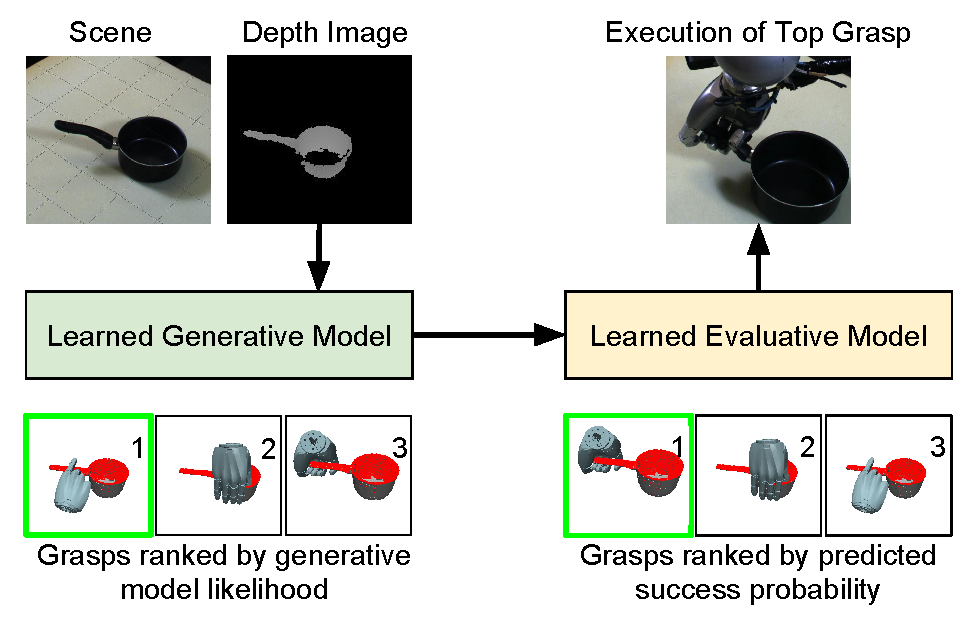
\includegraphics[width=\columnwidth]{images/contribution.pdf}
  \end{center}
  \caption{The basic architecture of a generative-evaluative learner. When shown a novel object the learned generative model (GM) produces many grasps according to its likelihood model. These are then each evaluated by a learned evaluative model (EM), which predicts the probability of grasp success. The grasps are then re-ranked according to the predicted success probability and the top ranked grasp is executed.}
\label{fig:systemArchitecture}
\end{figure}
Either or both a {\em generative} or {\em evaluative} model may be learned. If only a generative model is learned then evaluation must be carried out using mechanically informed reasoning, which, as we noted, cannot easily be applied to the case of novel objects seen from a single view. If only an evaluative model is learned then grasp generation must proceed by search. This is challenging for true dexterous grasping as the hand may have between nine and twenty actuated degrees of freedom. Thus, for dexterous grasping of novel objects from a single view, it becomes appealing to {\em learn} both the generative and the evaluative model. 

The contributions of this paper are as follows. First, we present a data-set of two million dexterous grasps in simulation that may be used to evaluate dexterous grasping algorithms. Second, we present a generative-evaluative architecture that combines data efficient learning of the generative model with data intensive learning in simulation of an evaluative model. Third, we present multiple variations of the evaluative model. Fourth, we present an extensive evaluation of all these models on our simulated data set. Fifth, we compare the two most promising variants on a real robot with a data-set of objects in challenging poses.

The model variants are organised in three dimensions. First, we employ two different generative models (GM1 \cite{kopicki2015ijrr} and GM2 \cite{kopicki2019ijrr}), one of which (GM2) is designed specifically for single view grasping. Second, we employ two different back-bones for the evaluative model based on VGG-16 and ResNet-50. Third, we experiment with two optimisation techniques--gradient ascent (GA) and stochastic annealing (SA)--to search for better grasps using the evaluative model as an objective function.

%The first contribution of this paper is the first generative-evaluative architecture where both generative and evaluative models are learned. Second, three novel evaluative networks, based on existing VGG-16 and ResNet-50 architectures, were proposed. Finally, a grasp simulation dataset containing 2M+ grasps on 295 objects, along with the simulator code will be released to to the community. In order to simulate the wide range of physical variations that real world objects have, a data set is acquired by simulation of  grasps proposed by the generative models on novel objects. We vary the physical characteristics of the objects in each simulated scene (mass, friction) which the robot can not observe. This dataset was used to train three evaluative neural networks. The evaluative models were then used to rank grasps produced by the generative models (GM1 and GM2) in real robot experiments. 

%The paper builds upon two existing generative grasp models that are learned from a small number of demonstrated grasps using the data-efficient method for LfD. Unlike other approaches to deep grasping, which are restricted to power-grasps, the methods are able to perform a wide variety of grasps, including pinch, rim, power, and handle grasps, and to use additional fingers to provide bracing.

The paper is structured as follows. First, we discuss related work. Second, the basic generative model is described in detail and the main features of the extended generative model are sketched. Third, we describe the design of the grasp simulation, the generation of the data set. Fourth, we describe the different architectures employed for the evaluative model. Fifth we describe the training of the evaluative model, the optimisation variants for the evaluative model and the simulated experimental study. Finally, we present the real robot study.
